
%%%%%%%%%%%%%%%%%%%%%%%%%%%%%%%%%%%%%%%%%%%%%%%%%%%%%%%%%%%%%%%%%%%%%%%%%
%           Capítulo 3: Diseño e implemantacion                         %
%%%%%%%%%%%%%%%%%%%%%%%%%%%%%%%%%%%%%%%%%%%%%%%%%%%%%%%%%%%%%%%%%%%%%%%%%

\chapter{Diseño del experimento}

\\
El desarrollo de la aplicación considera las siguientes situaciones para considerar un sistema útil para el manejo de almacenes. Dentro de las características útiles se menciona los siguientes puntos.

\begin{enumerate}
\item Registro de usuarios
\item Modificación de Almacenes
\item Modelamiento de productos
\end{enumerate}

Entre las características principales de un sistema de gestión de almacenes están los siguientes puntos.

\begin{enumerate}
\item Códigos de barras
\item Herramientas de informes
\item Previsión de inventarios
\item Alertas de inventarios
\end{enumerate}

%%%%%%%%%%%%%%%%%%%%%%%%%%%%%%%%%%%%%%%%%%%%%%%%%%%%%%%%%%%%%%%%%%%%%%%%%
%                          Modelamiento de Almacenes                    %
%%%%%%%%%%%%%%%%%%%%%%%%%%%%%%%%%%%%%%%%%%%%%%%%%%%%%%%%%%%%%%%%%%%%%%%%%
\section{Modelamiento de los almacenes}

\\
Dentro de un contexto variado de empresas, lo normal es dividirlas en dos grupos y que son empresas dedicadas a la fabricación y empresas dedicadas al comercio. De estos dos grupos de empresas, la gestión de almacenes es diferente. La gestión de almacenes en empresas dedicadas a la fabricación debe de considerarse un flujo interno que describa los movimientos de los materiales internamente para su transformación. Sin embargo tanto para la empresa dedicada a la fabricación de productos como a una empresa dedicada al comercio, ambos tienes que gestionar almacenes para la venta; en el caso de la primera esta gestión será para los productos terminados y una empresa comercial, le interesará la gestión de sus mercaderías a la venta.\\

En el siguiente listado se muestra un resumen de las necesidades para una empresa de fabricación y una dedicada al comercio. [\citep{PCD:2019:Online}]

\begin{enumerate}
\item PARA FABRICACIÓN
\begin{enumerate}
\item Seguimiento de materiales
\item Niveles de inventario para piezas y productos terminados
\item Re-ordenación automática
\item Integración ERP
\end{enumerate}
\item PARA ALMACENES
\begin{enumerate}
\item Sistema de códigos de barras avanzado (QR, y demás)
\item Soporte a ubicación múltiple
\item Sistema de seguimiento de estantería
\item Soporte de selección de pedidos
\end{enumerate}
\end{enumerate}

Cabe aclarar que el listado anterior no implica una necesidad en cada uno de los tipos de empresas ya que cada empresa puede prescindir de alguna de ellas, claro que esto también implicaría un costo asociado.

%%%%%%%%%%%%%%%%%%%%%%%%%%%%%%%%%%%%%%%%%%%%%%%%%%%%%%%%%%%%%%%%%%%%%%%%%
%                          Modelado                                     %
%%%%%%%%%%%%%%%%%%%%%%%%%%%%%%%%%%%%%%%%%%%%%%%%%%%%%%%%%%%%%%%%%%%%%%%%%
\section{Modelamiento de usuario}

El funcionamiento de sistemas en línea es el usuario el elemento por donde la aplicación funciona. Si bien no se está creando un sistema de gestión de usuarios, se debe modelar un correcto uso de recursos en función al usuario.\\

Un sistema en línea, debe proveer las opciones para que un usuario cualquiera pueda acceder a él. Para tal efecto es importante crear mecanismos de registro, con validación para que el usuario pueda registrarse y acceder a sus recursos.\\

El registro no debe ser complejo ni tomar mucho tiempo. Desde este punto de vista, el usuario debe registrar sus datos básicos, como ser su nombre y su correo electrónico. Estos datos son almacenado y además es importante que el usuario ingrese una clave de acceso, la que llamaremos “Password”. Muchos sistemas, realizan comprobaciones para que el “Password” de usuario sea lo más seguro, tanto para el usuario como para el sistema mismo.\\

De los detalles anteriores, se deriva los siguientes diagramas que modelan el usuario en el sistema.

\begin{figure}
  \centering
    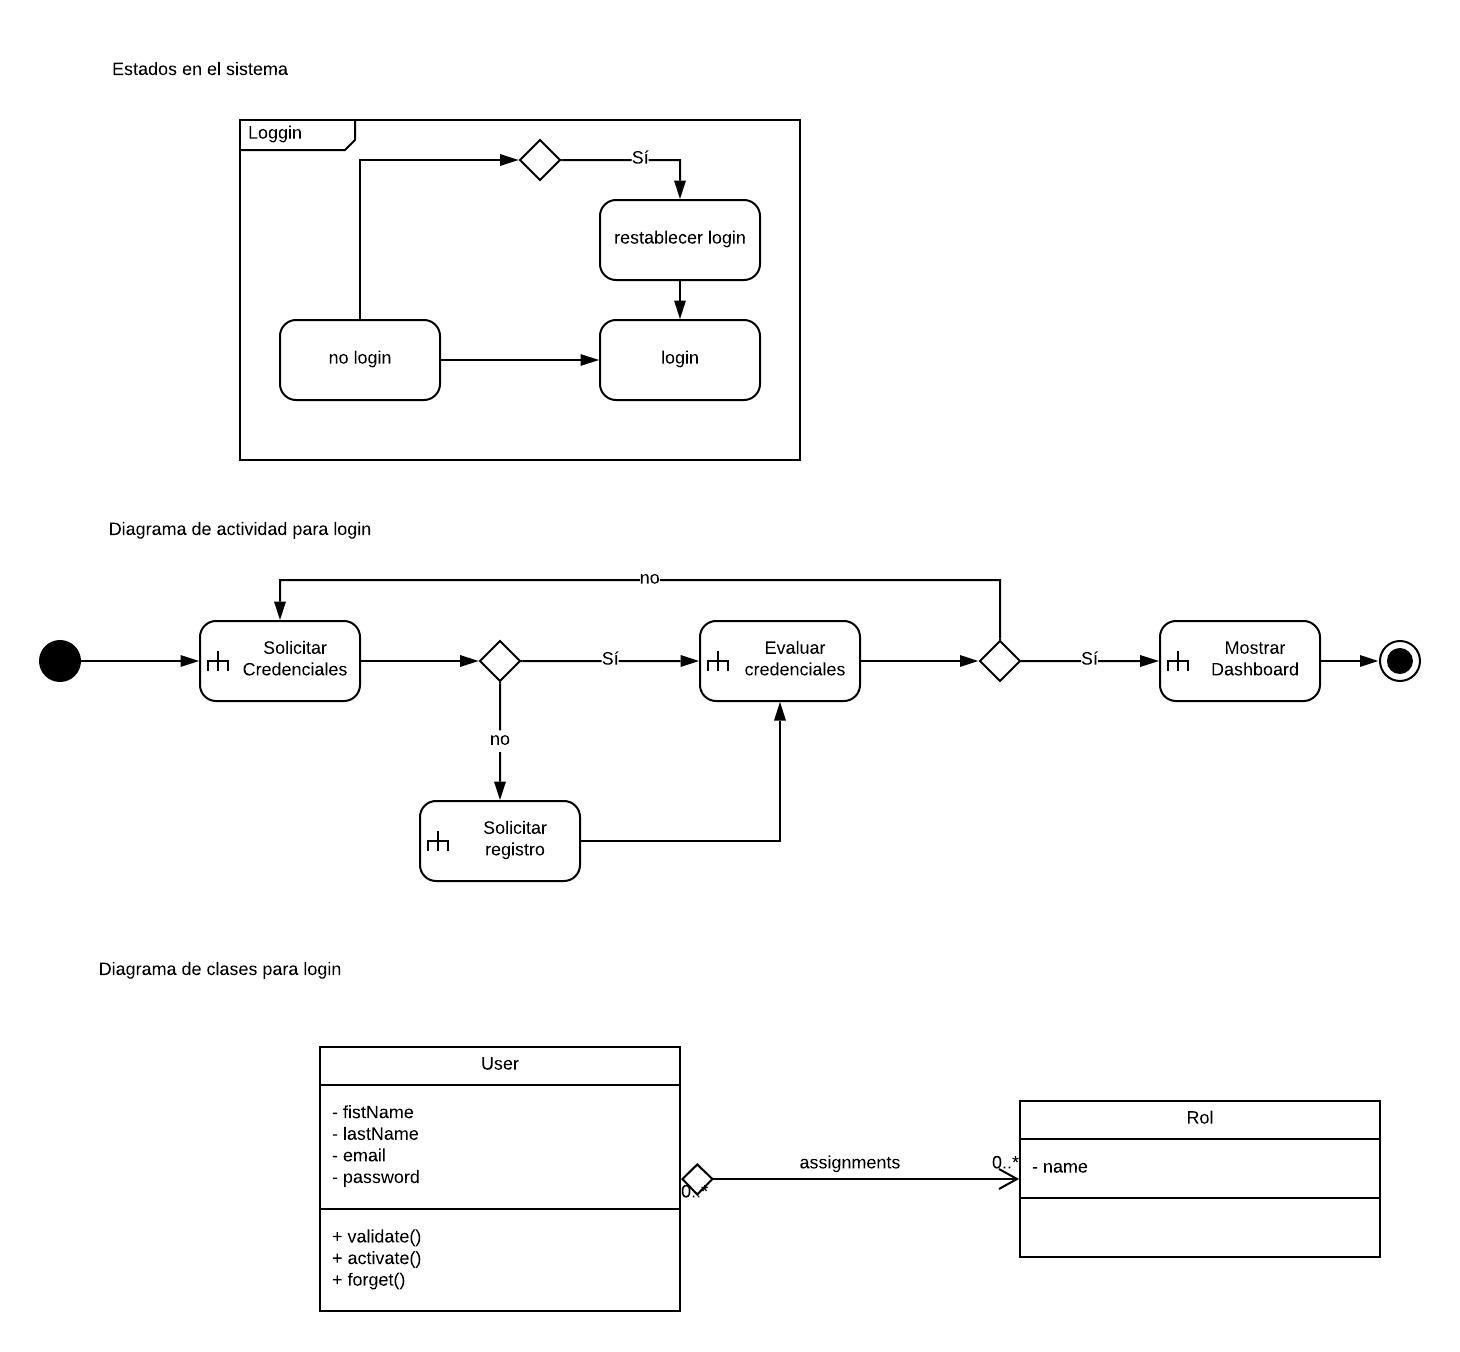
\includegraphics[scale=0.7]{./Capitulo3/figs/ADDStock-user-login.jpeg}
  \caption{Diagrama de estados, diagrama de actividades y diagrama de clases para el modelamiento de usuarios en el sistema de gestión de almacenes.}
  \label{user_login}
\end{figure}

El funcionamiento de manejo de usuarios en el sistema, se basa en el concepto de roles, lo cual permite al sistema manejar opciones. La división por roles nos permite definir accesos a diferentes opciones en el sistema. Para el propósito del sistema de gestión de almacenes, lo importante es permitir al usuario mismo, proteger su información de usuarios con menos privilegios que están encargados de tareas más concretas dentro de un sistema de almacenes.\\

La estructura de roles básicos que se puede manejar en el sistema son los siguientes:

\begin{itemize}
\item Superadmin
\item Admin
\item User
\begin{itemize}
\item Vendedor
\item Almacenero
\end{itemize}
\end{itemize}

El listado anterior muestra una estructura básica, ya que la idea es permitir al usuario crear más usuarios con roles que el mismo usuario pueda definir y por lo tanto los accesos que puedan tener a los recursos que vaya creando el usuario.\\

Se ha tomado pequeñas funciones que todos los sistemas de usuarios manejan y son la recuperación de “Password” de usuario y la mantención de sesión.

\subsection{La persistencia de la información}

En cuanto a la persistencia de la información, debe de realizarse ciertas consideraciones. Primeramente el motor de base de datos ideal será un sistema relacional, cabe considerar la existencia de motores no relacionales. En el mundo de motores relacionales esta los sistemas PostgreSQL, MySQL, Oracle, Microsoft SQL entre otros. Para los sistemas no relacionales tenemos los motores MongoDB, Redis, Elasticseach entre otros.

\begin{table}[htdp]
\centering
\begin{tabular}{||c | c | c ||}
\hline
\hline
\textbf{-} & \textbf{Database} & \textbf{Tipo} \\
\hline
\hline
1 & Oracle & Relational DBMS \\
\hline
\hline
2 & MySQL & Relational DBMS \\
\hline
\hline
3 & Microsoft SQL Server & Relational DBMS \\
\hline
\hline
4 & PostgreSQL & Relational DBMS \\
\hline
\hline
5 & MongoDB & Document store \\
\hline
\hline
6 & IBM Db2 & Relational DBMS \\
\hline
\hline
7 & Redis & Key-value store \\
\hline
\hline
8 & Elasticsearch & Search engine \\
\hline
\hline
9 & Microsoft Access & Relational DBMS \\
\hline
\hline
10 & SQLite & Relational DBMS \\
\hline
\hline
\end{tabular}
\caption[Para el mes de enero de 2019`]{Los 10 motores de bases de datos más populares. \\ Fuente https://fyaromo.com.co/2019/01/30/los-motores-de-bases-de-datos-mas-populares-relacionales-y-nosql/}
\label{tab:tabla-db-list} 
\end{table}
Fuente https://fyaromo.com.co/2019/01/30/los-motores-de-bases-de-datos-mas-populares-relacionales-y-nosql/

El objetivo de esta sección es poder seleccionar un motor de base de datos que puede trabajar de la mejor manera y permita un mejor desempeño y un mejor manejo de los datos. Por lo tanto, entre las características necesarias del sistema están listadas a continuación.

\begin{itemize}
\item Gran capacidad de almacenamiento.
\item Extensibilidad.
\item Escalabilidad.
\item Seguridad.
\item Optimizado para la búsqueda.
\item Resistencia ante los fallos.
\end{itemize}

Como puede observase en la Tabla \ref{tab:tabla-db-list}, esta tabulada mediante sus propiedades de ser un motor de base de datos relacional o no. Aunque no define ninguno de los atributos mencionados en la lista anterior. 

\section{Modelamiento de la empresa}

El sistema define la existencia de una empresa con cada cuenta de usuario. De este modo, se tiene una restricción de una empresa por cuenta creada. Sin embargo cada empresa puede tener definido varios usuarios, por lo cual haremos uso de los roles para definir una cuenta principal, que estará a cargo de la empresa y de los usuarios de esta misma.\\

El modelamiento general estará basado en una sola clase, que manejará la información de la empresa.\\

\begin{figure}
  \centering
    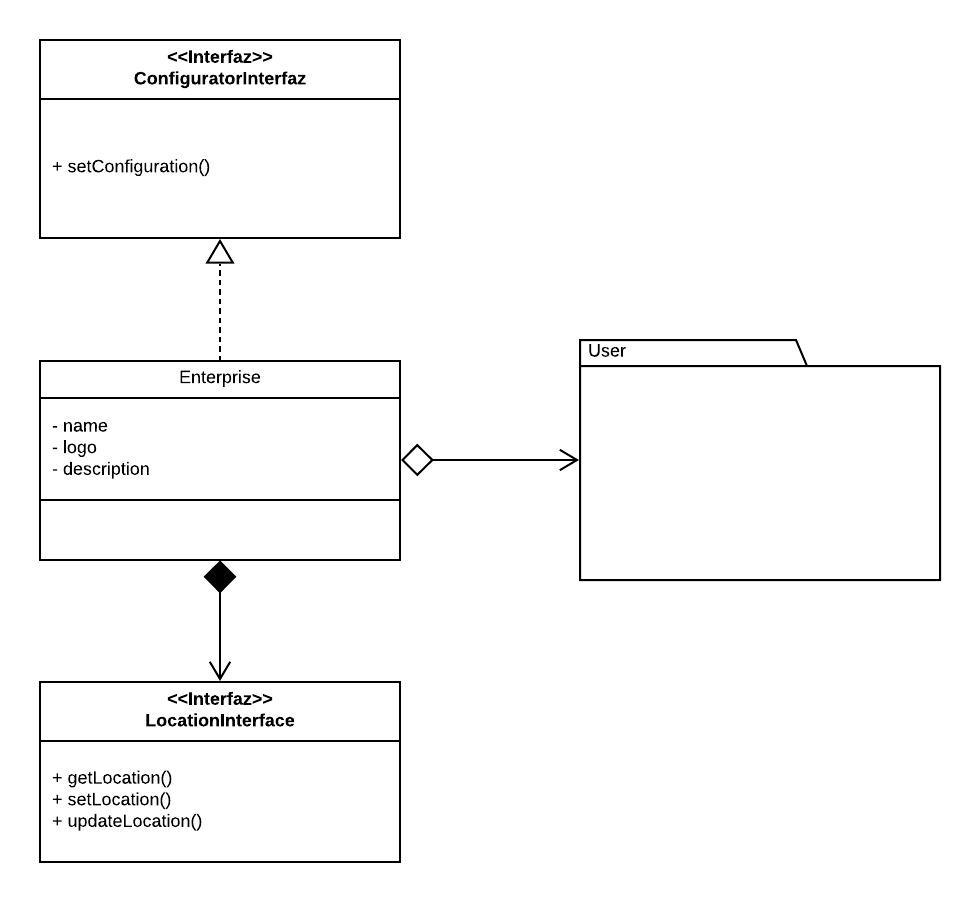
\includegraphics[scale=0.9]{./Capitulo3/figs/ADDStock-enterprise.jpeg}
  \caption{Diagrama de clases para el modelamiento de empresa.}
  \label{enterprise}
\end{figure}

La definición de empresa se basa en la información que se requiere guardar y esencialmente se trata del nombre de la empresa y su dirección. Cabe mencionar que la información tiene que ser guardada y está íntimamente ligada a las configuraciones que haya a realizarse en la aplicación.\\

En el modelo (figura \ref{enterprise}) presentado se trata de especificar que la clase empresa interviene en las configuraciones que se realizarán en la aplicación. Mediante el objeto empresa se realizará las configuraciones en la aplicación.\\

Este modelo mostrado en \ref{enterprise} requiere una explicación de porqué se está usando una \textbf{interface} para la localización. La idea general de localización está muy ligada a los almacenes, ya que se puede definir sucursales, puntos de donde los proveedores se encuentren y varios productos pueden estar en distintos lugares para su almacenado.

La información que será necesaria almacenar esta representada en el diagrama \ref{ER-diagram-v1}.

\section{Modelando el producto}

El producto es el tema principal de la aplicación y la información circulara en función a los productos que se tengan almacenados o en proceso. Incluso los productos que sean considerados de distinta manera, como por ejemplo los materiales, suministros, estos a su vez pueden tener un grado más de especialización ya que pueden ser materiales de transformación, materiales de uso como son los consumibles.\\

En este modelamiento todavía no se tomará en cuenta los movimientos de productos en almacenes ni su almacenamiento propiamente dicho.\\

La necesidad de información que hasta ahora se ha modelado corresponde a la figura \ref{Product-classes}

\begin{figure}
  \centering
    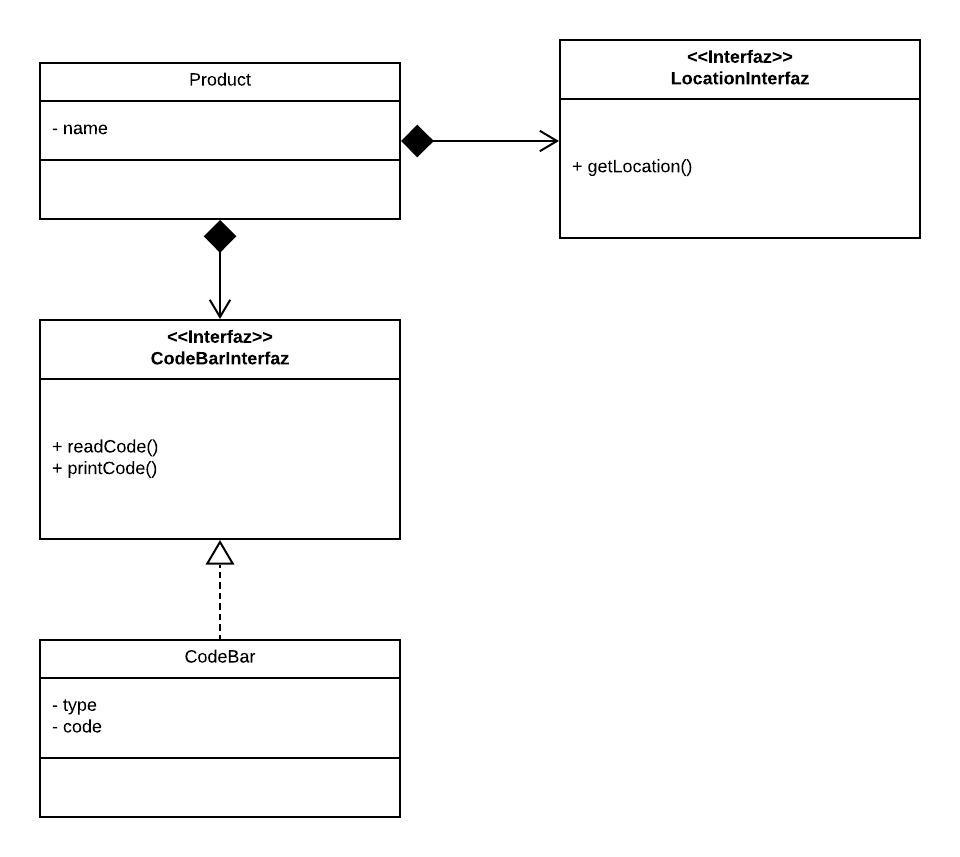
\includegraphics[scale=0.9]{./Capitulo3/figs/ADDStock-Product.jpeg}
  \caption{Diagrama de clases para el modelamiento de producto.}
  \label{Product-classes}
\end{figure}

La información general del producto viene dada por los valores de (name, description, price). Esta tupla de valores refleja la información de un producto que se podría manejar en una empresa.\\

Para el propósito del modelamiento y de la utilidad para la empresa en el manejo de un producto para almacenes es necesario considerar más valores. Para este propósito se elaboró una lista que describe a un producto.

\begin{itemize}
\item Nombre del producto.
\begin{itemize}
\item El producto puede ser vendido.
\item El producto puede ser comprado.
\end{itemize}
\item Tipo del producto.
\item Categoría.
\item Referencia interna. (Código o identificación interna)
\item Código de barras.
\item Notas internas.
\item Precio Venta. Considere las unidades de la moneda.
\item Costo.
\item Inventario. Información referida a lugar donde esta almacenado el producto, además de la ruta que sigue el producto dentro de la empresa.
\item Logística.
\begin{itemize}
\item Responsable. Este valor es un usuario del sistema que pertenece a la empresa.
\item Peso.
\item Volumen.
\item Plazo de entrega del cliente.
\end{itemize}
\item Descripción para pedidos de entrega
\item Descripción para Recepciones
\end{itemize}

\subsection{Operaciones}

Las operaciones que son útiles dentro una empresa en cuanto a los productos o materiales son los siguientes:

\begin{enumerate}
\item Transferencias.
\item Reposición.
\item Ajustes de inventario.
\item Desechar.
\item Ejecutar planificador.
\end{enumerate}

Las operaciones listadas anteriormente son básicas y están orientadas a realizar 1) movimientos dentro la empresa con el fin de que estén disponibles donde se los necesite y sean útiles. 2) Las reposiciones representan las reglas para mantener un número de productos disponibles dentro los almacenes. 3) El ajuste de inventario representa la actividad de contar las unidades físicas de cada producto que esta registrado en el sistema; por lo que representa un control vital. Suele efectuarse cada periodo de tiempo que la empresa vea necesario. 4) Desechar significa que el producto en si, tiene algún defecto, da{o, deterioro y que ya no puede ser usado, dentro del ciclo del procesos en la empresa. 5) Todo lo anterior tiene como objetivo mantener un control automático, en ese sentido el sistema procede a realizar los controles y las notificaciones que el usuario haya indicado.\\

Un punto también importante en un sistema de gestión de almacenes es la capacidad de ser configurable. Esto significa que dentro del sistema se tiene las opciones de cambiar ciertos valores que al usuario le interese y se adapte mejor a sus necesidades.\\

En este punto se detalla los siguientes valores como configurables:

\begin{itemize}
\item Unidades monetarias.
\item Unidades de peso y volumen.
\item Categorías de los productos.
\item formato de fecha y hora
\end{itemize}

Cabe aclarar que puede existir algún valor que el usuario necesita que sea configurable; para ello el uso del sistema permitirá identificar este requerimiento. Sin embargo esto escapa un poco del alcance de este proyecto. Eso es un tema de mantenimiento.

\subsection{Modelamiento de la información del Producto}

La sección anterior es una descripción de las necesidades de un sistema de almacenes para manejar los productos. En esta sección la idea principal es obtener los diagramas para identificar las clases que están involucradas y que permitirán el funcionamiento del sistema. En un primer nivel de formulación para una solución mediante un diagrama de clases se presenta en la figura \ref{Product-classes-v2}.

\begin{figure}
  \centering
    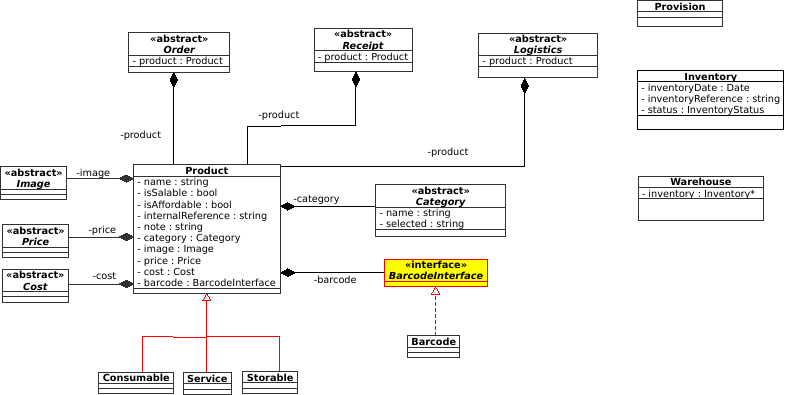
\includegraphics[scale=0.7]{./Capitulo3/figs/ADDStock-product-v2.png}
  \caption{Diagrama de clases para el modelamiento de producto en su segunda versión. En este diagrama se muestra las relaciones con los conceptos de Recepciones y Adquisiciones.}
  \label{Product-classes-v2}
\end{figure}

La idea general de esta propuesta de diseño (Figura \ref{Product-classes-v2}), se centra en la construcción de la clase \textit{Product}. El producto esta definido por atributos de clases y además tiene dependencias de las clases: \textit{Image}, \textit{Price}, \textit{Cost}, \textit{Category} y \textit{Bardcode}. Esta configuración trata de adaptar el patrón Builder, para lo cual se ha definido las dependencias de \textit{Product} como \textbf{asbtract} de esta manera sus clases concretas podrán ser manejadas por los métodos \textit{getProduct()} y \textit{buildPart()}. Los métodos mencionados anteriormente, son parte de la propuesta del patrón \textbf{Builder}. Este texto no tratará el patrón \textbf{Builder}, pero, se intentará explicarlo a lo largo del desarrollo de este capítulo.\\

Un segundo nivel de refinamiento se puede ver en la siguiente figura \ref{Product-classes-v3}.

\begin{figure}
  \centering
    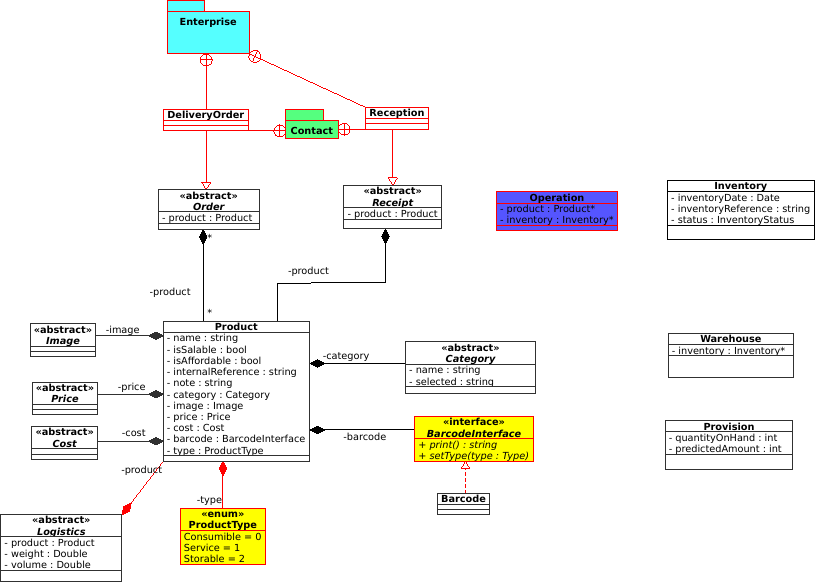
\includegraphics[scale=0.7]{./Capitulo3/figs/ADDStock-product-v3.png}
  \caption{Diagrama de clases para el modelamiento de producto en su tercera versión. En este diagrama se muestra las relaciones con las clases \textbf{abstract} y sus relaciones con otros módulos, como por ejemplo el módulo \textit{Enterprise}.}
  \label{Product-classes-v3}
\end{figure}

En la siguiente sección se desarrollará el diagrama de entidad-relación para el almacenamiento de los datos.

\section{Modelamiento Entidad-Relación}

Las secciones anteriores nos permite realizar un análisis de la interacción para generar un proceso. En el desarrollo del proceso, se genera información de forma de datos, que deben ser guardados.

Los datos generados en los procesos deben de guardarse, y para ello se modelará el sistema orientado a una base de datos relacional. Como se pudo observar en la tabla \ref{tab:tabla-db-list}, existe una variedad de motores de base de datos relacionales. Sin embargo, el sistema en desarrollo debe de escogerse un motor de base de datos que permita su funcionamiento.

La elección de una base de datos no es parte de este capítulo, por lo que nos centraremos en un modelamiento de base de datos en un alto nivel.

\begin{figure}
  \centering
    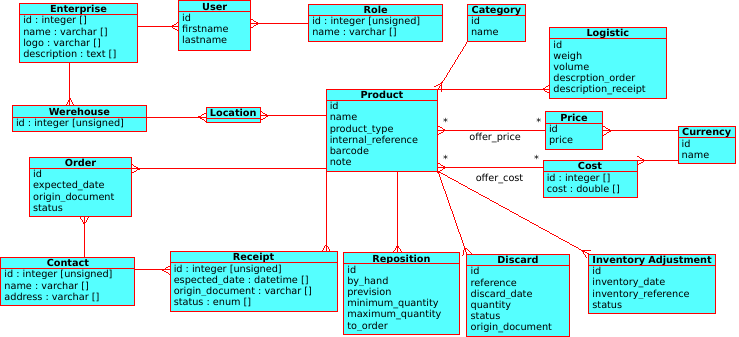
\includegraphics[scale=0.7]{./Capitulo3/figs/ADDStock-ER-diagram-v1.png}
  \caption{Diagrama Entidad-Relación. En este diagrama se muestra la relación que hay entre las distintas entidades que el sistema hará uso. La entidad que mas refleja relaciones es \textit{Product}. En esta entidad se ha tratado de establecer todos los atributos necesarios para su almacenaje en base de datos. Por otra parte cada entidad presenta ya un conjunto de atributos que se harán uso en el sistema.}
  \label{ER-diagram-v1}
\end{figure}

En el diagrama \ref{ER-diagram-v1}, se presenta una primera aproximación para el modelamiento de la información. Las entidades que se han podido definir en este diagrama son los siguientes:

\begin{itemize}
\item Category
\item Contact
\item Cost
\item Currency
\item Discard
\item Enterprise
\item Inventory\_Adjustment
\item Location
\item Logistic
\item Order
\item Price
\item Product
\item Receipt
\item Reposition
\item Role
\item User
\item Werehouse
\end{itemize}

Esta lista preliminar funcionará como punto de partida para hacer funcionar una primera versión del sistema de almacenes. Por lo tanto, el código que se generará de este diagrama, podrá ser subido a un motor de base de datos. Esta tarea se mostrará en el siguiente capítulo.
